\documentclass[oneside,a4paper,14pt]{extarticle}
\usepackage[a4paper,top=20mm,bottom=20mm,left=20mm,right=10mm]{geometry}
\usepackage[russian]{babel}
\usepackage{indentfirst}
\usepackage{graphicx}
\usepackage{caption}
\usepackage{titlesec}
\usepackage{ulem}
\usepackage{minted, fancyvrb}
\usepackage{tocloft}
\usepackage{hyperref}
\usepackage{microtype}

% Настройки заголовков без номеров
\titleformat{\section} {\normalsize\bfseries} {} {0em} {}
\titleformat{\subsection} {\normalsize\bfseries} {} {0em} {}
\titleformat{\subsubsection} {\normalsize\bfseries} {} {0em} {}

% Убираем номера в содержании
\renewcommand{\thesection}{}
\renewcommand{\thesubsection}{}
\renewcommand{\thesubsubsection}{}

% Интервал и абзац
\renewcommand\baselinestretch{1.45}\normalsize
\setlength{\parindent}{1.25cm}

% Настройки содержания
\renewcommand{\cftsecleader}{\cftdotfill{\cftdotsep}}
\setlength{\cftbeforesecskip}{5pt}
\renewcommand{\cftsecfont}{\normalfont} % Обычный шрифт для разделов в содержании
\renewcommand{\cftsecpagefont}{\normalfont} % Обычный шрифт для номеров страниц

\begin{document}

% Титульная страница (как в вашем оригинале)
\newpage
\thispagestyle{empty}
\begin{center}
    МИНИСТЕРСТВО НАУКИ И ВЫСШЕГО ОБРАЗОВАНИЯ РОССИЙСКОЙ ФЕДЕРАЦИИ ФЕДЕРАЛЬНОЕ ГОСУДАРСТВЕННОЕ БЮДЖЕТНОЕ ОБРАЗОВАТЕЛЬНОЕ УЧРЕЖДЕНИЕ ВЫСШЕГО ОБРАЗОВАНИЯ\\
    «ВЯТСКИЙ ГОСУДАРСТВЕННЫЙ УНИВЕРСИТЕТ»\\
    (ВятГУ)
\end{center}

\vspace{5mm}

\begin{center}
    \textbf{ОТЧЁТ ПО УЧЕБНОЙ ПРАКТИКЕ}
\end{center}

\vspace{1cm}

\begin{center}
  \uline{\hfill\textit{Черкасов Александр Андреевич}\hfill}
  \par
  \footnotesize \textit{(Ф.И.О. обучающегося)}
\end{center}
\begin{center}
	\textit{09.03.01 Информатика и вычислительная техника}\\
	\uline{\hfill\textit{Инженерия программного и аппаратного обеспечения}\hfill}
  \par
  \footnotesize \textit{(направление подготовки (специальность), направленность(профиль))}
\end{center}

\noindent
\begin{tabular}{lc}
	Место прохождения практики: & \uline{\hfill \textit{ФГБОУ ВО <<ВятГУ>>, кафедра ЭВМ} \hfill} \\
    & \footnotesize\textit{(наим. организации, структурного подразделения организации)}
\end{tabular}

\vspace{2cm}
\noindent
\begin{tabular}{lccc}
  \multicolumn{4}{l}{Итоговая оценка: \uline{\hfill}} \\
    Руководитель \\
  практики от университета & \uline{\hfill \textit{12.07.2025} \hfill} & \uline{\hspace{4cm}} & \uline{\hspace{4cm}} \\
    & \footnotesize\textit{(дата)} & \footnotesize\textit{(подпись)} & \footnotesize\textit{(Ф.И.О.)}
\end{tabular}

\vspace{4cm}

\begin{center}
    Киров, 2025 г.
\end{center}

\newpage
\tableofcontents
\thispagestyle{plain}

\clearpage

\section{Введение}


Учебная практика проходила на базе ФГБОУ ВО «Вятский государственный университет» в период с 30.06.2025 по г. 13.07.2025.
Цель практики: закрепление знаний, умений и навыков полученных на первом курсе.\\
\textbf{Задачи практики:}
\begin{itemize}
  \item[$-$] Решение общих задач научно-исследовательского характера, предполагающих поиск ответа ближайшего к оптимальному в условиях ограничения временных ресурсов
  \item[$-$] Индивидуальное задание по разработке графического приложения
\end{itemize}

\clearpage

\section{Общаяя часть}

В данном разделе рассматриваются вопросы, связанные с прохождением общей для всех обучающихся части практики.

\subsection{Первое задание: Обнаружение чёрных квадратов на изображении}

\sloppy В заданном графическом файле содержится изображение с чёрными квадратами, обладающими следующими свойствами:

\begin{itemize}
    \item[$-$] Фиксированный размер одного чёрного квадрата: $20\times20$ пикселей
    \item[$-$] Псевдослучайное расположение с ограничением: площадь пересечения с существующими квадратами $\leq 30\%$ при добавлении
    \item[$-$] Наличие искажений и шумов
\end{itemize}

\noindent\textbf{Алгоритм:}
\begin{enumerate}
    \item \textbf{Предобработка:} Конвертация в градации серого и бинаризация с пороговым значением для выделения чёрных объектов
    \item \textbf{Поиск контуров:} Примененение алгоритма обнаружения границ.
    \item \textbf{Фильтрация квадратов:} Аппроксиммация контуров полигонами, отбор объектов с 4 вершиами, проверка соотношения сторон (0.9-1.1) и фильтрация по размеру квадрата ($20 \times 20 \pm$ погрешность)
    \item \textbf{Визуализация:} Отрисовка рамок вокруг обнаруженных квадратов с нумерацией
\end{enumerate}

\clearpage

\subsection{Второе задание: Поиск делителей большого числа}

\textbf{Цель:} Найти все положительные делители большого числа ($\leq10000$).\\

\noindent\textbf{Алгоритм:}
\begin{enumerate}
    \item \textbf{Факторизация:}
    \begin{itemize}
        \item[$-$] Решето Эратосфена для простых чисел ($\leq 10^6$)
        \item[$-$] Алгоритм Полларда-Ро для больших делителей
        \item[$-$] Тест Миллера-Рабина для проверки простоты
    \end{itemize}
    \item \textbf{Генерация делителей:}
    \begin{itemize}
        \item[$-$] Для чисел с ($\leq10^4$) делителей: полный перебор комбинаций простых множителей
        \item[$-$] Для чисел с ($>10^4$) делителей: приоритетная очередь для генерации наименьших 9999 делителей
    \end{itemize}
    \item \textbf{Оптимизации:}
    \begin{itemize}
        \item[$-$] Длинная арифметика с базой $10^9$ (BigInt)
        \item[$-$] Алгоритм Карацубы для быстрого умножения
        \item[$-$] Модульное возведение в степень
    \end{itemize}
\end{enumerate}

\clearpage

\subsection{Третье задание: Раскраска графа}

\textbf{Цель:} Минимизировать количество цветов для правильной раскраски графа.\\

\noindent\textbf{Алгоритм DSATUR:}
\begin{enumerate}
    \item \textbf{Инициализация:}
    \begin{itemize}
        \item[$-$] $degree[i]$ — степень вешины $i$
        \item[$-$] $neigh\_colors[i]$ — множество цветов соседей
        \item[$-$] $used[i]$ - отметка о раскраске
    \end{itemize}
    \item \textbf{Выбор вершины:} Максимальная насыщенность (размер $neigh\_colors$) или степень. Если несколько вершин, выбираем с наибольшей степенью.
    \item \textbf{Раскраска:} Минимальный отсутствующий цвет в $neigh\_colors$
    \item \textbf{Обновление:} Добавление цвета в $neigh\_colors$ соседей
\end{enumerate}

\clearpage

\subsection{Четвёртое задание: Покрытие бинарной матрицы}

\textbf{Цель:} Минимизировать количество прямоугольников для покрытия однородных областей.\\

\noindent\textbf{Жадный алгоритм:}
\begin{enumerate}
    \item \textbf{Обход матрицы:} Сверху вниз, слева направо с пропуском покрытых ячеек
    \item \textbf{Построение прямоугольника:}
    \begin{itemize}
        \item[$-$] Определение базового значения (0 или 1)
        \item[$-$] Расширение вправо до границы значения
        \item[$-$] Расширение вниз c проверкой столбцов
    \end{itemize}
    \item \textbf{Пометка покрытия:} Регистрация координат прямоугольника и пометка этих ячеек как покрытых
\end{enumerate}

\clearpage

\section{Вывод по общей части}

В ходе выполнения общей части практики были успешно решены четыре алгоритмические задачи различной сложности. Основные достижения и наблюдения:

\begin{enumerate}
    \item \textbf{Эффективность алгоритмов}:
    \begin{itemize}
        \item[$-$] Для задач обработки изображений (1) и матричных операций (4) оптимальны пошаговые методы с линейной сложностью
        \item[$-$] Комбинированные подходы (детерминированные + вероятностные) эффективны для факторизации больших чисел (2)
        \item[$-$] Эвристики (DSATUR) дают хорошие результаты для NP-трудных задач (3)
    \end{itemize}
    
    \item \textbf{Технические сложности}:
    \begin{itemize}
        \item[$-$] Обработка зашумленных изображений
        \item[$-$] Реализация длинной арифметики для чисел $>10^{100}$
        \item[$-$] Оптимизация памяти при генерации делителей
    \end{itemize}
    
    \item \textbf{Практическая значимость}:
    \begin{itemize}
        \item[$-$] Освоение методов компьютерного зрения
        \item[$-$] Разработка оптимизированных структур данных
        \item[$-$] Реализация алгоритмов для больших чисел
    \end{itemize}
\end{enumerate}

Решения демонстрируют высокую эффективность: все задачи решены в рамках ограничений с минимальной вычислительной сложностью, что подтверждает корректность выбранных подходов.

\clearpage

\section{Индивидуальное задание}

В рамках индивидуального задания была разработана простая головоломка под названием \textbf{Ternary Tiles}, вдохновлённая механикой игры <<2048>>. Однако в отличие от классического аналога, в данной реализации используются степени тройки, а числа могут быть как положительными, так и отрицательными.

Цель игры — достичь клетки со значением определённой степени по модулю (например, $81$ или $81n$), комбинируя плитки с одинаковыми модулями. Размер игрового поля зависит от выбранной сложности: $3\times3$, $4\times4$ или $5\times5$.

\subsection{Описание игрового процесса}

\sloppy Каждая плитка имеет значение вида $3^n$, где $n$ — целое число (в том числе отрицательное). Плитки могут быть положительными ($3^n$) или отрицательными ($-3^n$), и они равноправны: при создании новой плитки шанс получить положительное или отрицательное значение одинаков.\\

\noindent\textbf{Правила слияния:}
\begin{itemize}
    \item[$-$] Сливаются только плитки с одинаковыми модулями.
    \item[$-$] Если у сливаемых плиток одинаковый знак, степень увеличивается на 1.
    \item[$-$] Если знаки противоположные, степень уменьшается на 1.
    \item[$-$] Если результатом слияния становится степень ноль ($3^0 = 1$), плитка исчезает.
\end{itemize}

\noindent\textbf{Пример:}
\begin{itemize}
    \item[$-$] $3$ и $3 \Rightarrow 9$
    \item[$-$] $3$ и $-3 \Rightarrow 1$, затем исчезает
    \item[$-$] $9$ и $-9 \Rightarrow 3$
\end{itemize}

Игровая логика строится так, что игроку приходится внимательно следить не только за величинами плиток, но и за их знаками. Игнорирование отрицательных плиток может привести к потере прогресса и понижению степени уже собранного значения. (Рисунки 1.1 и 1.2 иллюстрируют игровой процесс на разных уровнях сложности.)

\begin{figure}[H]
	\centering
	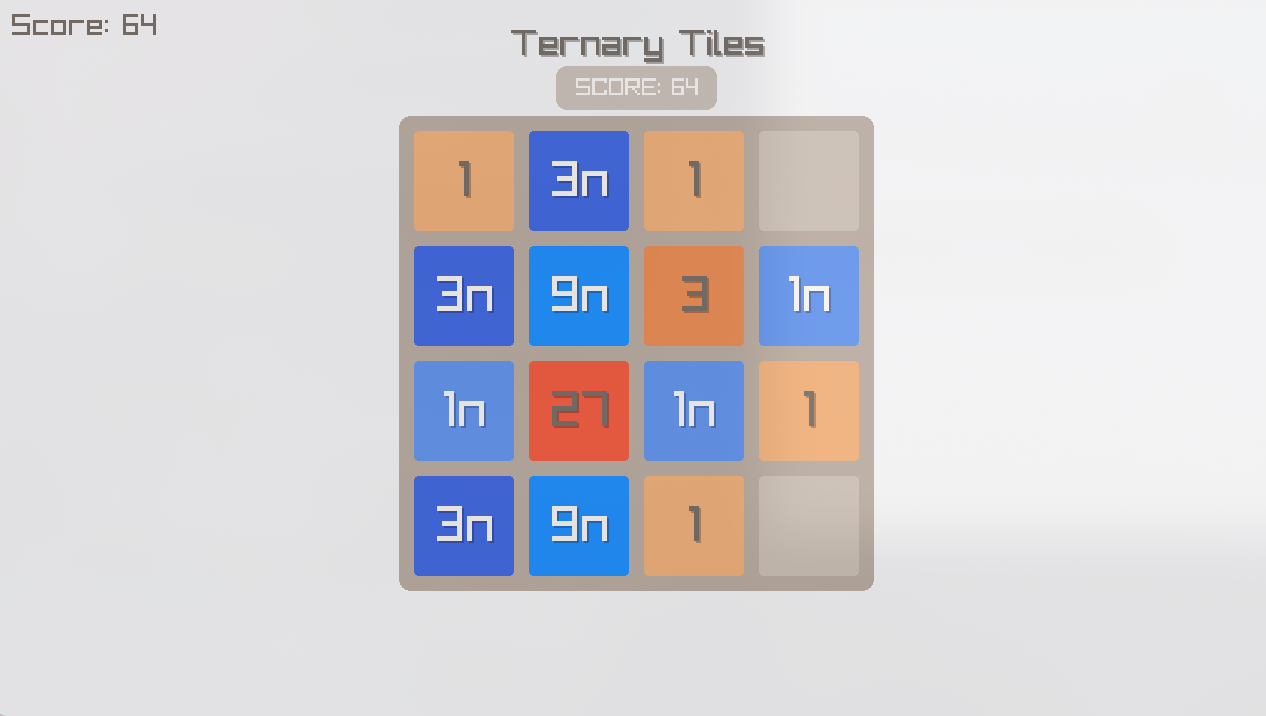
\includegraphics[width=0.9\textwidth]{pics/screen4x4.png}
	\caption*{Рисунок 1.1 - Игровой процесс на базовой сложности с полем 4x4.}
\end{figure}

\begin{figure}[H]
	\centering
	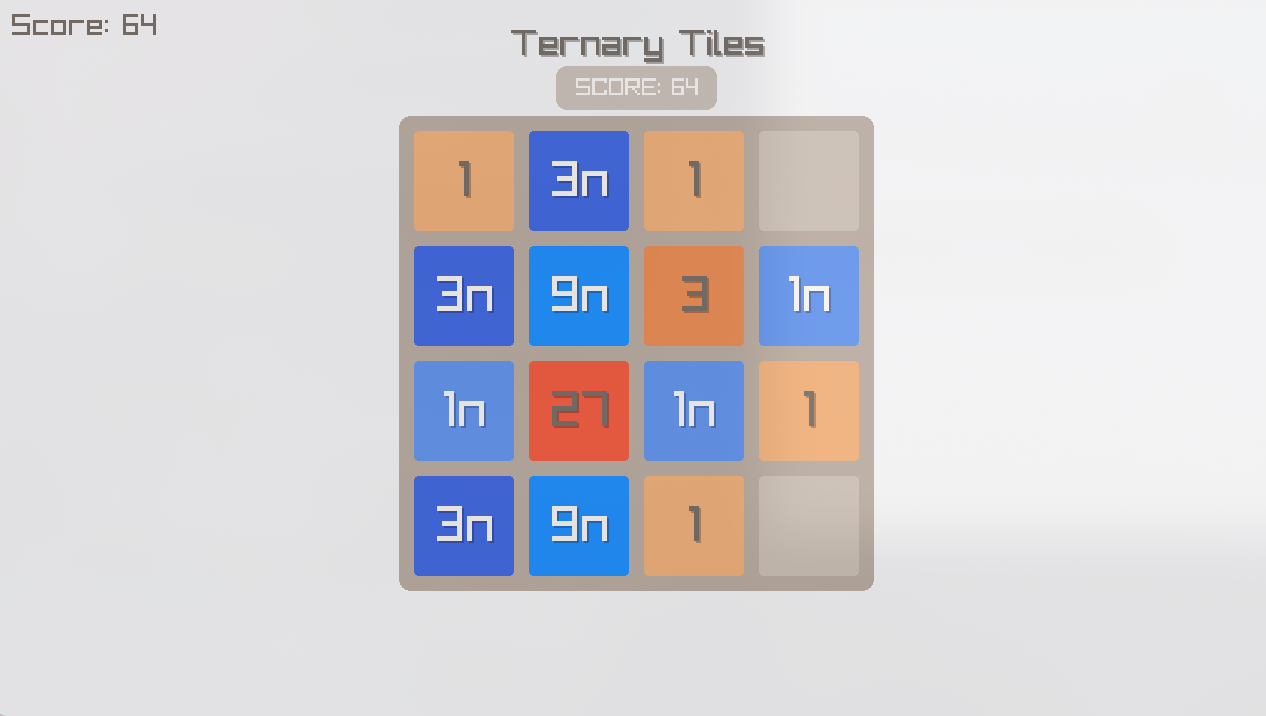
\includegraphics[width=0.9\textwidth]{pics/screen4x4.png}
	\caption*{Рисунок 1.2 - Игровой процесс на максимальной сложности с полем 5x5.}
\end{figure}

\begin{figure}[H]
	\centering
	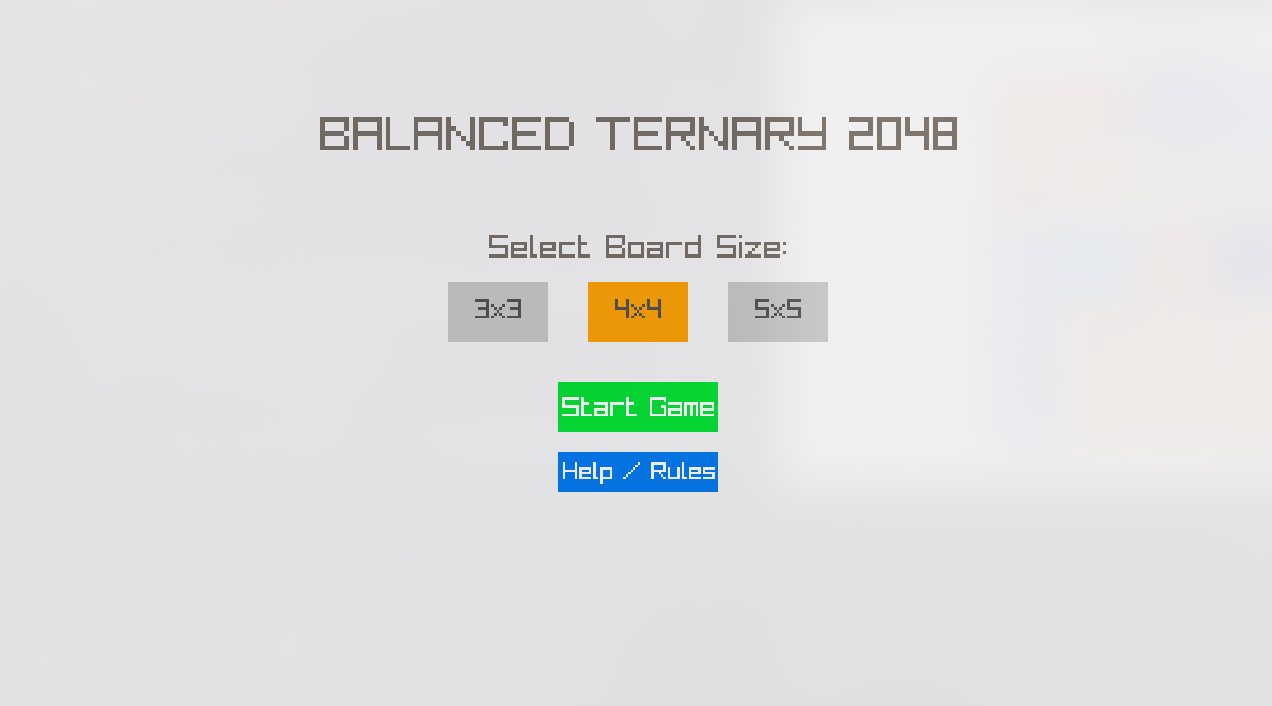
\includegraphics[width=0.9\textwidth]{pics/menu.png}
	\caption*{Рисунок 1.3 - Главное меню игры.}
\end{figure}

\clearpage

\subsection{Используемые технологии}

Для реализации проекта применялись следующие инструменты:

\begin{itemize}
    \item[$-$] \textbf{C++17} — основной язык программирования. Используется стандартная библиотека STL (векторы, уникальные указатели, алгоритмы) и современный стиль разработки: RAII, умные указатели, scoped enums и другие конструкции.
    
    \item[$-$] \textbf{Raylib} — кроссплатформенная C-библиотека для разработки графических приложений. Использовалась для:
    \begin{itemize}
        \item[$-$] отображения игрового поля и плиток;
        \item[$-$] обработки ввода с клавиатуры;
        \item[$-$] рендеринга текста и графических объектов;
    \end{itemize}

    \item[$-$] \textbf{OpenGL (через Raylib)} — графический API, лежащий в основе Raylib, используется для рендеринга.

    \item[$-$] \textbf{Meson + Ninja} — система сборки. Позволяет быстро и удобно конфигурировать проект и производить инкрементальную сборку. Пример конфигурационного файла Meson представлен ниже:

\begin{minted}{meson}
project('TernaryTiles', 'cpp',
  default_options: ['cpp_std=c++17'])

raylib_dep = dependency('raylib', required: true)

executable('ternary_tiles',
  'src/main.cpp',
  dependencies: raylib_dep)
\end{minted}

\end{itemize}

\subsection{Результат}

Разработанное приложение представляет собой минималистичную, но интересную головоломку, позволяющую в простой форме изучить механизмы взаимодействия данных, рендеринга и пользовательского ввода. Несмотря на малый объём, проект демонстрирует основы построения графических приложений, включая игровую логику, управление ресурсами, и сборку.

\clearpage

\section{Вывод}

Учебная практика позволила применить на практике ключевые знания, полученные в течение первого курса, в контексте решения прикладных и исследовательских задач. Были успешно выполнены как общие, так и индивидуальные задания, охватывающие различные аспекты программной инженерии.

В результате прохождения практики:

\begin{itemize}
\item[$-$] Закреплены навыки анализа и реализации алгоритмов обработки данных, компьютерного зрения и комбинаторики;
\item[$-$] Получен практический опыт в проектировании и разработке настольного приложения на C++ с использованием библиотеки Raylib;
\item[$-$] Освоена система сборки Meson, обеспечивающая гибкость и масштабируемость проекта;
\item[$-$] Улучшены навыки структурирования и документирования кода;
\item[$-$] Получено понимание принципов взаимодействия пользовательского интерфейса с логикой приложения.
\end{itemize}

В рамках индивидуального проекта удалось реализовать полноценную головоломку с уникальной игровой механикой, что продемонстрировало способность к проектированию и реализации нестандартных решений. Практика прошла продуктивно и дала мощный стимул для дальнейшего профессионального роста.

\newpage

\setminted{style = rainbow_dash, fontsize = \small}

\section{Приложение А1. Исходный код индивидуального задания}
\inputminted{cpp}{ternary_tiles/src/main.cpp}

\clearpage

\section{Приложение А2. Исходный код индивидуального задания}
\inputminted{cpp}{ternary_tiles/include/Game/Renderer.hpp}

\clearpage

\section{Приложение А3. Исходный код индивидуального задания}
\inputminted{cpp}{ternary_tiles/src/Game/Renderer.cpp}

\clearpage

\section{Приложение А4. Исходный код индивидуального задания}
\inputminted{cpp}{ternary_tiles/include/Game/GameBoard.hpp}

\clearpage

\section{Приложение А5. Исходный код индивидуального задания}
\inputminted{cpp}{ternary_tiles/src/Game/GameBoard.cpp}

\clearpage

\section{Приложение А6. Исходный код индивидуального задания}
\inputminted{cpp}{ternary_tiles/include/Game/BalancedTernary.hpp}

\clearpage

\section{Приложение А7. Исходный код индивидуального задания}
\inputminted{cpp}{ternary_tiles/src/Game/BalancedTernary.cpp}

\clearpage

\section{Приложение А8. Исходный код индивидуального задания}
\inputminted{cpp}{ternary_tiles/include/Game/Tile.hpp}

\clearpage

\section{Приложение А9. Исходный код индивидуального задания}
\inputminted{meson}{ternary_tiles/meson.build}

\end{document}